\documentclass{beamer}
\usetheme{metropolis}

\usepackage[spanish]{babel}
\usepackage[utf8]{inputenc}
\usepackage{graphicx}
\usepackage{tikz}
\usepackage{xcolor}
\usepackage{amsmath}
\usepackage{listings}
\usepackage{fontawesome}

\usetikzlibrary{positioning,shapes.multipart,calc,arrows,shapes.geometric}

% Definición de colores personalizados
\definecolor{primary}{RGB}{46, 204, 113}
\definecolor{secondary}{RGB}{52, 152, 219}
\definecolor{accent}{RGB}{231, 76, 60}
\definecolor{background}{RGB}{236, 240, 241}
\definecolor{gradient1}{RGB}{255, 107, 107}
\definecolor{gradient2}{RGB}{255, 159, 67}

% Configuración del tema
\setbeamercolor{normal text}{fg=black,bg=background}
\setbeamercolor{structure}{fg=primary}
\setbeamercolor{alerted text}{fg=accent}

\definecolor{lightgray}{rgb}{0.95,0.95,0.95}
\definecolor{darkgreen}{rgb}{0,0.5,0}
\definecolor{darkblue}{rgb}{0,0,0.5}

\lstset{
  backgroundcolor=\color{lightgray},
  basicstyle=\tiny\ttfamily,
  keywordstyle=\color{darkblue}\bfseries,
  commentstyle=\color{darkgreen},
  stringstyle=\color{red},
  numbers=left,
  numberstyle=\tiny\color{gray},
  stepnumber=1,
  numbersep=5pt,
  showspaces=false,
  showstringspaces=false,
  showtabs=false,
  frame=single,
  tabsize=2,
  language=Python,
  breaklines=true,
  breakatwhitespace=true
}

\title{\Huge\textbf{Visualización de Datos}}
\author{Analítica de Datos}
\date{}

\begin{document}

\begin{frame}
    \titlepage
    \begin{tikzpicture}[remember picture,overlay]
        \node[anchor=south west,inner sep=30pt] at (current page.south west) {
            \includegraphics[height=1cm]{../misc/UdeSA.png}
        };
    \end{tikzpicture}
\end{frame}

\begin{frame}{Herramientas de visualización}
    \begin{center}
        \begin{tabular}{ccc}
            \begin{minipage}{2.5cm}
                \centering
                {\Large \faCode}\\[0.1cm]
                \textbf{Matplotlib}\\[0.1cm]
            \end{minipage} &
            \begin{minipage}{2.5cm}
                \centering
                {\Large \faImage}\\[0.1cm]
                \textbf{Seaborn}\\[0.1cm]
            \end{minipage} &
            \begin{minipage}{2.5cm}
                \centering
                {\Large \faTable}\\[0.1cm]
                \textbf{Pandas}\\[0.1cm]
            \end{minipage}
        \end{tabular}
        
        \vspace{0.8cm}
        
        \begin{tabular}{cc}
            \begin{minipage}{2.5cm}
                \centering
                {\Large \faGlobe}\\[0.1cm]
                \textbf{Plotly}\\[0.1cm]
            \end{minipage} &
            \begin{minipage}{2.5cm}
                \centering
                {\Large \faDesktop}\\[0.1cm]
                \textbf{Tableau}\\[0.1cm]
            \end{minipage}
        \end{tabular}
    \end{center}
\end{frame}

\begin{frame}{Kokemone}
    \begin{center}
        \url{https://www.youtube.com/watch?v=B_JMyKEQQ1E}
    \end{center}
\end{frame}

\begin{frame}[fragile]{Configuración inicial}
\begin{lstlisting}[numbers=left, numbersep=5pt]
# Importar librerias necesarias
import pandas as pd
import matplotlib.pyplot as plt
import seaborn as sns

# Configurar estilo de seaborn
sns.set_style('whitegrid')

# Cargar datos
df = pd.read_csv('Pokemon.csv', index_col=0)
\end{lstlisting}
\end{frame}

\begin{frame}{Análisis exploratorio inicial}
    \begin{columns}
        \begin{column}{0.8\textwidth}
            \begin{itemize}
                \item<1->[{\makebox[1em][c]{\textcolor{black}{\faInfo}}}] \textbf{df.info()} - Información del dataset
                \item<2->[{\makebox[1em][c]{\textcolor{black}{\faList}}}] \textbf{df.head()} - Primeras filas
                \item<3->[{\makebox[1em][c]{\textcolor{black}{\faCalculator}}}] \textbf{df.describe()} - Estadísticas descriptivas
                \item<4->[{\makebox[1em][c]{\textcolor{black}{\faColumns}}}] \textbf{df.shape} - Dimensiones
                \item<5->[{\makebox[1em][c]{\textcolor{black}{\faExclamationTriangle}}}] \textbf{df.isnull().sum()} - Valores faltantes
            \end{itemize}
        \end{column}
        \begin{column}{0.2\textwidth}
            \centering
            {\fontsize{60}{60}\selectfont \faSearch}
        \end{column}
    \end{columns}
\end{frame}

\begin{frame}[fragile]{Información del dataset}
    \begin{lstlisting}[numbers=left, numbersep=5pt]
# Informacion del dataset
df.info()

# Resultado:
# Index: 151 entries, 1 to 151
# Data columns (total 12 columns):
# 0   Name       151 non-null    object
# 1   Type 1     151 non-null    object
# 2   Type 2     67 non-null     object
# 3   Total      151 non-null    int64
# 4   HP         151 non-null    int64
# 5   Attack     151 non-null    int64
# 6   Defense    151 non-null    int64
# 7   Sp. Atk    151 non-null    int64
# 8   Sp. Def    151 non-null    int64
# 9   Speed      151 non-null    int64
# 10  Stage      151 non-null    int64
# 11  Legendary  151 non-null    bool
    \end{lstlisting}
\end{frame}

\begin{frame}[fragile]{Estadísticas descriptivas}
    \begin{lstlisting}[numbers=left, numbersep=5pt]
# Estadisticas descriptivas
df.describe()

# Muestra:
# - count: cantidad de valores no nulos
# - mean: promedio
# - std: desviacion estandar
# - min: valor minimo
# - 25%: primer cuartil
# - 50%: mediana
# - 75%: tercer cuartil
# - max: valor maximo
    \end{lstlisting}
\end{frame}

\begin{frame}{Scatter Plot - Relación entre variables}
    \begin{center}
        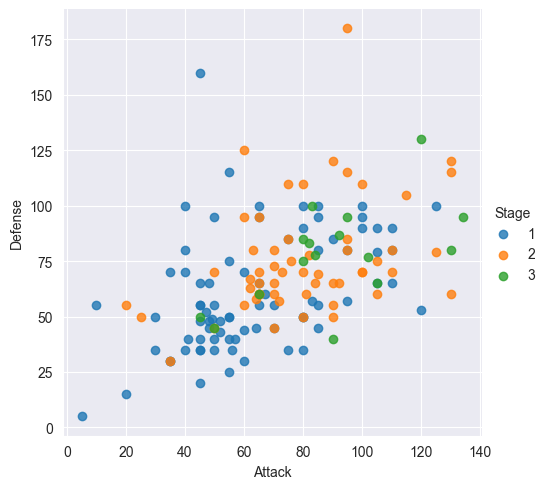
\includegraphics[width=0.5\textwidth]{img/scatter.png}
        
        \begin{itemize}
            \item Muestra la relación entre dos variables numéricas
            \item Permite identificar correlaciones
            \item Útil para detectar outliers
            \item Puede incluir una línea de regresión
        \end{itemize}
    \end{center}
\end{frame}

\begin{frame}[fragile]{Creando scatter plots}
\begin{lstlisting}[numbers=left, numbersep=5pt]
# Scatter plot basico
sns.lmplot(x='Attack', y='Defense', data=df)

# Sin linea de regresion
sns.lmplot(x='Attack', y='Defense', data=df,
           fit_reg=False)

# Con colores por categoria
sns.lmplot(x='Attack', y='Defense', data=df,
           fit_reg=False, hue='Stage')

# Ajustando limites de ejes
plt.ylim(0, 200)
plt.xlim(0, 160)
    \end{lstlisting}
\end{frame}

\begin{frame}{Box Plot - Distribución de datos}
    \begin{center}
        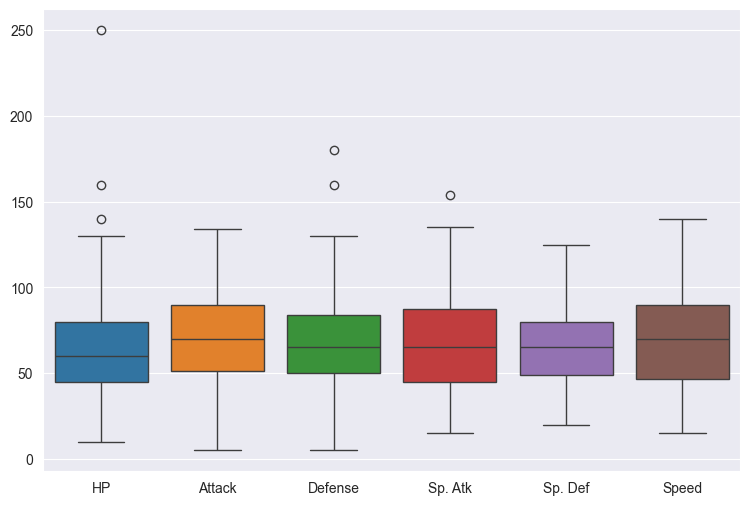
\includegraphics[width=0.5\textwidth]{img/boxplot.png}
        
        \begin{itemize}
            \item Muestra la distribución de datos
            \item Identifica outliers
            \item Compara grupos
            \item Muestra mediana, cuartiles y rango
        \end{itemize}
    \end{center}
\end{frame}

\begin{frame}[fragile]{Box plots con seaborn}
\begin{lstlisting}[numbers=left, numbersep=5pt]
# Box plot de todas las variables
plt.figure(figsize=(9,6))
sns.boxplot(data=df)

# Solo variables numericas relevantes
stats_df = df.drop(['Total', 'Stage', 'Legendary'], axis=1)
plt.figure(figsize=(9,6))
sns.boxplot(data=stats_df)
\end{lstlisting}
\end{frame}

\begin{frame}{Heatmap - Matriz de correlación}
    \begin{center}
        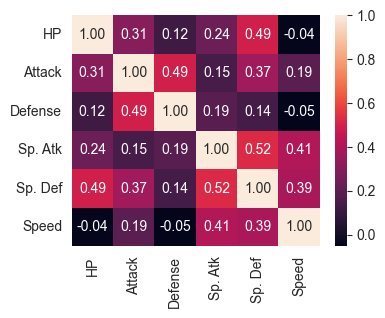
\includegraphics[width=0.5\textwidth]{img/heatmap.png}
        
        \begin{itemize}
            \item Muestra correlaciones entre variables
            \item Colores indican intensidad
            \item Útil para identificar patrones
            \item Valores de -1 a +1
        \end{itemize}
    \end{center}
\end{frame}

\begin{frame}[fragile]{Creando heatmaps}
\begin{lstlisting}[numbers=left, numbersep=5pt]
# Calcular correlacion
corr = stats_df.select_dtypes(include='number').corr()

# Heatmap basico
plt.figure(figsize=(4,3))
sns.heatmap(corr, annot=True, fmt='.2f')

# Con paleta de colores
sns.heatmap(corr, cmap='coolwarm')

# Con centro en 0
sns.heatmap(corr, cmap='coolwarm', center=0)

# Con limites especificos
sns.heatmap(corr, cmap='coolwarm', center=0, 
            vmin=-1, vmax=1)
\end{lstlisting}
\end{frame}

\begin{frame}{Terminamos}
    \begin{center}
        \Large{\textbf{¿Dudas?\\¿Consultas?}}
    \end{center}
    \begin{tikzpicture}[remember picture,overlay]
        \node[anchor=south,inner sep=30pt] at (current page.south) {
            \includegraphics[height=1cm]{../misc/UdeSA.png}
        };
    \end{tikzpicture}
\end{frame}

\end{document} 